\chapter{Introduction}

\graphicspath{{\dir/}}

Sequence alignment is a class of combinatorial problems that is of primary
importance for analysis of genetic data. Algorithms and tools for alignment have
been thoroughly developed and routinely used for genome assembly, RNA
quantification, detecting splicing, oncology, multiple sequence alignment (MSA),
and evolutionary biology. Types of sequence alignment include global alignment,
semi-global alignment, mapping, local alignment, and others. For each type, a
common tradeoff that had to be done is between the alignment accuracy and the
performance to find it. An additional difficulty is the fact that in the
upcoming pangenomic era, these algorithms must be also applicable to complex
graph structures. For more than 60 years, a linear sequence has been extremely
useful as a representation of a single genome. The affordability of sequencing
technologies enables not only to sequence genomes deeper but also to sequence
many genomes (e.g. of organisms or single cells), building a pangenome (an
abstracted genome that represents the genetic variation of a whole clade). The
shift towards population studies in the last decade motivates the adoption of
graph data structures which serve as compressed representations of collections
of related genomes (genomes are paths in the graph). During my PhD program, we
initiated a new direction of sequence alignment based on the informed shortest
path algorithms A* that we have shown to be both provably optimal, practically
scalable and more performant than existing aligners in certain cases. The
objective of this project is to develop our work on A* for sequence alignment
from prototypical to practical, which includes the development of algorithms,
formal proofs and software development. Our specific aim is to use the already
constructed base for the development of AStarix as an industrial-scale mapper
handling human-scale graph references, long and noisy reads, while being
competitive in runtime and memory even to suboptimal aligners. In order to
fulfill this aim, work in several directions will be needed: 1) rigorous
development of the seed heuristic theory, 2) theoretical analysis of the
expected runtime, 3) implementation optimized for runtime, memory,
parallelization and use-cases. Our vision is that A* could become the default
approach for sequence alignment, useful to the computational biology,
bioinformatics and the more general algorithmic community.

\label{ch:introduction}

%\section{Research goals and scope}
%\paragraph{Problem statement}
%\paragraph{Problem domain}

\section{Preliminaries}

\section{Current state of research in the field}

\begin{floatingfigure}[l]{0.5\textwidth}
    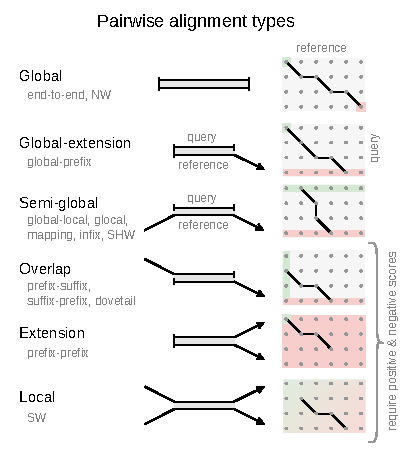
\includegraphics[width=0.5\textwidth]{alignment-types}
	\caption[Alignment types]{Alignment types.}
\end{floatingfigure}

Comparing one sequence to another is a basic combinatorial problem that has
several variations (shown on the right), each applicable in computational
biology. Needleman-Wunsch (1970)  and Smith-Waterman (1981) are dynamic
programming (DP) algorithms that serve as base solutions for global (or
computing edit distance of two strings) and semi-global alignments (or mapping
when a set of sequences is being aligned). Given that there is both biological
and technical variation in the data, a biologically plausible alignment is one
that minimizes the corresponding differences (e.g. insertions, deletions and
substitutions), so metrics based on edit distance are usually used. Backurs and
Indyk (2015) showed that even calculating the edit distance between two
sequences (without finding an alignment), is not generally solvable in
strongly-subquadratic time. Moreover, even for related sequences of lengths n
and m and edit distance s, the fastest optimal global (Marco-Sola et al., 2021;
Šošic and Šikic, 2017)) and semi-global aligners (Rautiainen et al., 2017) scale
quadratically when the edit distance increases with the length, which is the
case for sequencing errors and biological variation: O(s*min(n,m))=O(enm) and
O(nm), respectively, where e is the error rate (Navarro, 2001). In the age of
big data and long reads (e.g. PacBio, ONP), this quadratic scaling with length
is prohibitive, so the algorithms with practical usage (e.g. minimap2, bwt,
kallisto) do not guarantee optimality but run in subquadratic time (Kucherov,
2019). The gap between fast and optimal global alignment has been recognized but
no optimal algorithms are known that run subquadratically for related sequences
(Medvedev, 2022a). The interest towards genome graphs keeps increasing with the
first International Genome Graph Symposium being held this year in Ascona,
Switzerland (2022). The benefits of using graph references representing
biological variation has been demonstrated to increase the alignment quality
(Garrison et al., 2018). The transition towards graph references only aggravates
the computational issues owing to the potentially complex graph topology (Equi
et al., 2019). The optimal algorithms used in computational biology explore the
search space of possible alignments in an uninformed fashion: by aligning a
prefix of one sequence to a prefix of the other. This contrasts with the
informed search algorithms such as the algorithm by Hunt and Szymanski (1977)
solving the longest common subsequence (LCS) problem (a special case of the edit
distance alignment). Sequence alignment can naturally be formulated as a
shortest path problem solvable by Dijkstra’s algorithm (Ukkonen, 1985). A* is an
informed generalization of Dijkstra’s algorithm (Hart, 1968) but it has not been
successfully applied to sequence alignment. A* may be the missing piece in the
“a major open problem to implement an algorithm with linear-like empirical
scaling on inputs where the edit distance is linear in n” (Medvedev, 2022a).

\section{Global and semi-global alignment}

\section{Mapping to reference graphs}

\section{Alignment as shortest path}

\section{\A algorithm and its heuristic function} \label{sec:astar}

% paper: trie
\subsection{Background: General \A algorithm} \label{TRIEsubsec:general-astar}
Given a weighted graph $G=(V,E)$ with $E \subseteq V \times V \times
\mathbb{R}_{\geq 0}$, the \A algorithm (abbreviated as \A) searches for the
shortest path from sources $S \subseteq V$ to targets $T \subseteq V$. It is an
extension of \dijkstra's algorithm that additionally leverages a \emph{heuristic
function} $h \colon V \to \mathbb{R}_{\geq 0}$ to decide which paths to explore
first.
%
If $h(u) \equiv 0$, \A is equivalent to \dijkstra's algorithm.
%
You can refer to the \A and \dijkstra algorithms in \cref{alg:astar}, but do not
assume knowledge of either algorithm in the following.
%
At a high level, \A maintains the set of all \emph{explored} states, initialized
with the set of sources $S$. Then, \A iteratively \emph{expands} the explored
state with lowest estimated cost by exploring all its neighbors, until it finds
a target. Here, the cost for node $u$ is estimated by the distance from source, called $g(u)$, plus the estimate from the heuristic $h(u)$.

\para{Heuristic Function}
The heuristic function $h(u)$ estimates the
cost $h^*(u)$ of a shortest path in $G$ from $u$ to a target $t \in T$. Intuitively, a
good heuristic correlates well with the distance from $u$ to $t$.

To ensure that \A indeed finds the shortest path, $h$ should be
\emph{admissible}:

\begin{definition}[Admissible heuristic] A heuristic $h$ is \emph{admissible}
    if it provides a lower bound on the distance to the closest target: $\forall
    u. h(u) \leq h^*(u)$.
\end{definition}

While any admissible $h$ ensures that \A finds optimal
alignments~\cite{dechter_generalized_1985}, the specific choice of $h$
is critical for performance. In particular, decreasing the error $\delta(u) =
h^*(u)-h(u)$ can only improve the performance of
\A~\cite{dechter_generalized_1985}. Thus, a key contribution of ours is
a domain-specific heuristic $h$.


\para{\A algorithm}
We aim to guarantee optimal alignment while optimizing the average runtime
to not reach its worst-case complexity. While \dijkstra is an algorithm that
explores graph nodes in the order of their distance from the start, \A is a
generalization of \dijkstra that also accounts for their distance from the
target. \A prioritizes the exploration of nodes that seem to be closer to the
target nodes. This way, \A can sometimes dramatically improve on the performance
of \dijkstra while remaining optimal.

There has been one attempt to apply \A for optimal
alignment~\cite{dox2018efficient} which uses a heuristic function that accounts
only for the length of the remaining query sequence to be aligned. However, it
does not significantly outperform \dijkstra (in fact, it is equivalent for
a zero matching cost).
%
In contrast, the heuristic function we introduce is more informative and
consistently outperforms \dijkstra.

\cref{alg:astar} shows a generic implementation of the \A algorithm,
roughly following~\cite{dechter_generalized_1985}.
We do not implement the reconstruction of the best alignment in order to simplify the presentation.
The procedure \mbox{\textsc{BacktrackPath}} traces the best alignment back to the $source$, based on remembered edges used to optimize $f$ for each alignment state.
%
\cref{alg:astar} also shows a simple implementation of \dijkstra in terms of \A.
We omit the implementation of \textsc{BacktrackPath} for simplicity.

\begin{algorithm}[t]
	\caption{\A~algorithm} \label{alg:astar}
	\begin{algorithmic}[1]
		\Function{\A}{$G\colon \text{Graph}$,
			$S\colon \text{Sources}$,
			$T\colon \text{Targets}$,
			$h\colon \text{Heuristic function}$}
		\State $g \gets \mli{Map}\colon (\text{Nodes} \to \mathbb{R}_{\geq 0})$
		\Comment Shortest paths lengths to explored nodes

		\State $f \gets \mli{Map}\colon (\text{Nodes} \to \mathbb{R}_{\geq 0})$
		\Comment $f(u)=g(u)+h(u)$ 

		\State $Q \gets \mli{MinPriorityQueue}(\mli{priority}=f)$ 
		\Comment Priorities according to $f$
		\ForAll{$s \in S$}
			\State $g[s] \gets 0.0,\, f[s] \gets 0.0$
			\State $Q.\mli{push}(s)$
			\Comment Initially, explore all $s \in S$
		\EndFor
		\While{$Q \neq \emptyset$}
			\State $\mli{curr} \gets Q.\mli{pop}()$
			\Comment Get state with minimal $f$ to be expanded
			\If{$\mli{curr} \in T$}
				\State \Return \Call{BacktrackPath}{$\mli{curr}$}
				\Comment Reconstruct a walk to $\mli{curr}$
			\EndIf
			\ForAll{$(\mli{curr},\mli{next},\mli{cost}) \in G.\mli{outgoingEdges}(\mli{curr})$}
			\State $g_\mli{next} \gets g[\mli{curr}] + \mli{cost}$
			\State $\hat{f}_\mli{next} \gets g_\mli{next} + h(\mli{next})$
				\Comment Candidate value for $f[\mli{next}]$
				\If{$\hat{f}_\mli{next} < f[\mli{next}{}]$}
					\State $g[\mli{next}] \gets g_\mli{next}$		
					\State $f[\mli{next}] \gets \hat{f}_\mli{next}$		
					\State $Q.\mli{push}(\mli{next})$
					\Comment Explore state $\mli{next}$
				\EndIf
		\EndFor
		\EndWhile
		\State \textbf{assert} $\mli{False}$
		\Comment Cannot happen if $T$ is reachable from $S$
		\EndFunction

		\Statex

		\Function{\dijkstra}{$G\colon \mli{Graph}$,
			$S\colon \mli{Sources}$,
			$T\colon \mli{Targets}$}
			\State $h(v) \gets 0.0$
			\Comment Constant-zero function $h$
			\State $\Call{\A}{G,S,T,h}$
		\EndFunction
	\end{algorithmic}
\end{algorithm}

% paper: seeds

\subsection{\A~algorithm for finding a shortest path} \label{SEEDsec:astar}
%
The \A~algorithm is a shortest path algorithm that generalizes \dijkstra's
algorithm by directing the search towards the target.
Given a weighted graph $G=(V,E)$, the \A~algorithm finds a shortest path from
sources $S \subseteq V$ to targets $T \subseteq V$.
%
To prioritize paths that lead to a target, it relies on an admissible heuristic
function $h \colon V \to \mathbb{R}_{\geq 0}$, where $h(v)$ estimates the
remaining length of the shortest path from a given node $v \in V$ to a target
$t \in T$.


\para{Algorithm}
% 
In a nutshell, the \A~algorithm maintains a set of \emph{explored} nodes,
initialized by all possible starting nodes $S$. It then iteratively
\emph{expands} the explored state $v$ with lowest estimated total cost $f(v)$ by
exploring all its neighbors. Here, $f(v) := g(v) + h(v)$, where $g(v)$ is the
distance from $s \in S$ to $v$, and $h(v)$ is the estimated distance from $v$ to
$t \in T$.
%
When the \A~algorithm expands a target node $t \in T$, it reconstructs the path
leading to $t$ and returns it.
%
For completeness, \cref{SEEDapp:astar} provides an implementation of \A.

\para{Admissibility}
%
The \A~algorithm is guaranteed to find a shortest path if its heuristic $h$
provides a lower bound on the distance to the closest target, often referred to
as $h$ being \emph{admissible} or optimistic.

Further, the performance of the \A~algorithm relies critically on the choice of
$h$. Specifically, it is crucial to have low estimates for the optimal paths but
also to have high estimates for suboptimal paths.

\para{Discussion}
%
To summarize, we use the \A~algorithm to find a shortest path from $\st{u}{0}$
to $\st{v}{|q|}$ in $\AG$. To guarantee optimality, its heuristic function
$h\st{v}{i}$ must provide a lower bound on the shortest distance from state
$\st{v}{i}$ to a terminal state of the form $\st{w}{\lvert q \rvert}$.
%
Equivalently, $h\st{v}{i}$ should lower bound the minimal cost of aligning
$q[i{:}]$ to $\RG$ starting from $v$, where $q[i{:}]$ denotes the suffix of $q$
starting at position $i$ ($0$-indexed).
%
The key challenge is thus finding a heuristic that is not only admissible but
also yields favorable performance.

% paper:global
% Shortest paths, A* for MSA and semi-global alignment (AStarix), gaps
\paragraph{Shortest paths and \A}
A pairwise alignment that minimizes edit distance corresponds to a shortest path in the
\emph{edit graph}~\citep{vintsyuk1968speech,ukkonen1985algorithms}. Assuming
non-negative edit costs, a shortest path can be found using \dijkstra's
algorithm~\citep{ukkonen1985algorithms} (\cref{GLOBALfig1-dij}) or
\A~\citep{spouge1989speeding}. \A is an informed search algorithm which uses a
task-specific heuristic function to direct its search. Depending on the
heuristic function, a shortest path may be found significantly faster than by an
uninformed search such as \dijkstra's algorithm. In the context of semi-global
sequence-to-graph alignment, \A has been used to empirically scale sublinearly
with the reference size for short reads~\citep{ivanov2020astarix}.           %% HIGHER PRIORITY

\paragraph{Heuristic function}

\section{Contributions}

\paragraph{Tools}

\dictum[Freeman Dyson]{It is better to be wrong than to be vague.}
\vskip 1em
%\begin{otherlanguage}{ngerman}
%Die ältesten Bestimmungen der wahren Grösse der Moleküle hat die kinetische
%Theorie der Gase ermöglicht, während die an Flüssigkeiten beobachteten
%physikalischen Phänomene bis jetzt zur Bestimmung der Molekülgrössen nicht
%gedient haben. \dots
%\end{otherlanguage}



% Accuracy and Metrics
The number of possible alignments grow exponentially with length. The usual
underlying question to finding ``correct'' alignments. Regarding the precision
of alignment, one is usually interested in base-to-base (aka letter-to-letter)
correspondence between the sequences, even though for some applications a less
detailed solution is sufficient: only the similarity between sequences or the
location where a read maps to a reference. Exact alignment is only useful for
very short sequences (often kmers), and for all other cases the optimized metric
may be hamming distance, edit distance (unit costs), Levenshtein distance,
affine costs, convex and concave costs, general costs and others. 

% Problem statement
Depending on the the number of aligned sequences, there is pairwise alignment
and multiple sequence alignment (MSA). Depending on the parts of the sequences
that are aligned to each other, we differentiate global, local and various
semi-global alignemnts. There are generalizations to sequence-to-sequence
alignment, including aligning to nonlinear structures, such as directed acyclic
graphs, DAGs, general graphs and others. These structures are nowadays becoming
more common as a compressed form of representing a set of references to which a
sequence can be aligned. Often, one best alignment is sufficient but finding
several best (top-K) alignments. In the context of read mapping, a set of reads
is aligned to the same reference sequence so an indexing procedure is often
useful for the performance.

We specifically consider the mapping of a set of reads to a general graph, and
the global pairwise alignment.

Existing optimal algorithms are based on dynamic programming (DP) and
run in quadratic time (assuming that the number of errors is proportional to the
length)

we employ the A* algorithm which is an \emph{informed search} algorithm.
TODO: a case for the informed algorithms